\documentclass[14pt]{extbook}
\usepackage{multicol, enumerate, enumitem, hyperref, color, soul, setspace, parskip, fancyhdr} %General Packages
\usepackage{amssymb, amsthm, amsmath, bbm, latexsym, units, mathtools} %Math Packages
\everymath{\displaystyle} %All math in Display Style
% Packages with additional options
\usepackage[headsep=0.5cm,headheight=12pt, left=1 in,right= 1 in,top= 1 in,bottom= 1 in]{geometry}
\usepackage[usenames,dvipsnames]{xcolor}
\usepackage{dashrule}  % Package to use the command below to create lines between items
\newcommand{\litem}[1]{\item#1\hspace*{-1cm}\rule{\textwidth}{0.4pt}}
\pagestyle{fancy}
\lhead{Makeup Progress Quiz 3}
\chead{}
\rhead{Version B}
\lfoot{4315-3397}
\cfoot{}
\rfoot{Fall 2020}
\begin{document}

\begin{enumerate}
\litem{
Find the equation of the line described below. Write the linear equation as $ y=mx+b $ and choose the intervals that contain $m$ and $b$.\[ \text{Perpendicular to } 7 x - 6 y = 11 \text{ and passing through the point } (2, 10). \]\begin{enumerate}[label=\Alph*.]
\item \( m \in [-0.98, 0.42] \hspace*{3mm} b \in [11.46, 11.73] \)
\item \( m \in [-0.17, 1.98] \hspace*{3mm} b \in [8.11, 8.3] \)
\item \( m \in [-0.98, 0.42] \hspace*{3mm} b \in [7.93, 8.17] \)
\item \( m \in [-0.98, 0.42] \hspace*{3mm} b \in [-11.72, -11.48] \)
\item \( m \in [-1.88, -0.98] \hspace*{3mm} b \in [11.46, 11.73] \)

\end{enumerate} }
\litem{
Solve the equation below. Then, choose the interval that contains the solution.\[ -3(2x + 4) = -18(6x -17) \]\begin{enumerate}[label=\Alph*.]
\item \( x \in [2.99, 3.3] \)
\item \( x \in [2.29, 2.8] \)
\item \( x \in [-3.2, -2.71] \)
\item \( x \in [2.76, 2.93] \)
\item \( \text{There are no real solutions.} \)

\end{enumerate} }
\litem{
Solve the equation below. Then, choose the interval that contains the solution.\[ -3(-4x + 8) = -18(11x -10) \]\begin{enumerate}[label=\Alph*.]
\item \( x \in [0.96, 0.99] \)
\item \( x \in [0.73, 0.76] \)
\item \( x \in [0.77, 0.88] \)
\item \( x \in [-0.77, -0.61] \)
\item \( \text{There are no real solutions.} \)

\end{enumerate} }
\litem{
Solve the linear equation below. Then, choose the interval that contains the solution.\[ \frac{-4x + 7}{2} - \frac{-7x -9}{4} = \frac{-6x -8}{5} \]\begin{enumerate}[label=\Alph*.]
\item \( x \in [-3.8, -2.2] \)
\item \( x \in [-9.1, -7.2] \)
\item \( x \in [-27.2, -23.3] \)
\item \( x \in [-1.3, 1.6] \)
\item \( \text{There are no real solutions.} \)

\end{enumerate} }
\litem{
First, find the equation of the line containing the two points below. Then, write the equation as $ y=mx+b $ and choose the intervals that contain $m$ and $b$.\[ (-3, 3) \text{ and } (4, -2) \]\begin{enumerate}[label=\Alph*.]
\item \( m \in [-0.55, 1.13] \hspace*{3mm} b \in [-5.2, -4.73] \)
\item \( m \in [-0.83, 0.7] \hspace*{3mm} b \in [-7.08, -5.35] \)
\item \( m \in [-0.83, 0.7] \hspace*{3mm} b \in [0.04, 1.92] \)
\item \( m \in [-0.83, 0.7] \hspace*{3mm} b \in [-1.71, -0.3] \)
\item \( m \in [-0.83, 0.7] \hspace*{3mm} b \in [4.81, 7.7] \)

\end{enumerate} }
\litem{
Write the equation of the line in the graph below in Standard form $Ax+By=C$. Then, choose the intervals that contain $A, B, \text{ and } C$.
\begin{center}
    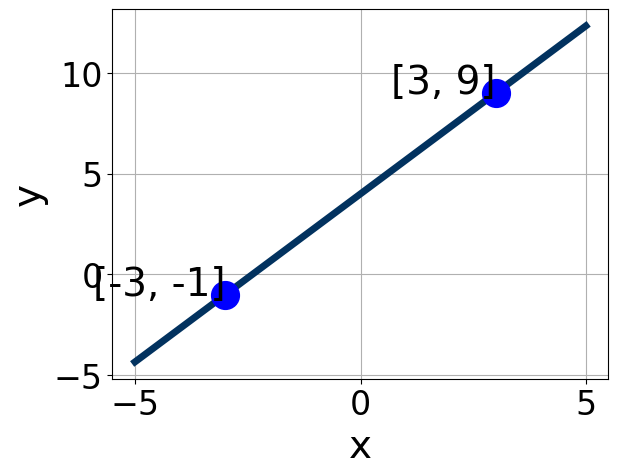
\includegraphics[width=0.5\textwidth]{../Figures/linearGraphToStandardCopyB.png}
\end{center}
\begin{enumerate}[label=\Alph*.]
\item \( A \in [1, 7], \hspace{3mm} B \in [-4.29, -2.06], \text{ and } \hspace{3mm} C \in [-14, -9] \)
\item \( A \in [-3.67, 1.33], \hspace{3mm} B \in [0.71, 1.08], \text{ and } \hspace{3mm} C \in [0, 7] \)
\item \( A \in [-3.67, 1.33], \hspace{3mm} B \in [-1.89, -0.45], \text{ and } \hspace{3mm} C \in [-8, 0] \)
\item \( A \in [1, 7], \hspace{3mm} B \in [2.38, 4.43], \text{ and } \hspace{3mm} C \in [9, 13] \)
\item \( A \in [-7, -4], \hspace{3mm} B \in [2.38, 4.43], \text{ and } \hspace{3mm} C \in [9, 13] \)

\end{enumerate} }
\litem{
Write the equation of the line in the graph below in Standard form $Ax+By=C$. Then, choose the intervals that contain $A, B, \text{ and } C$.
\begin{center}
    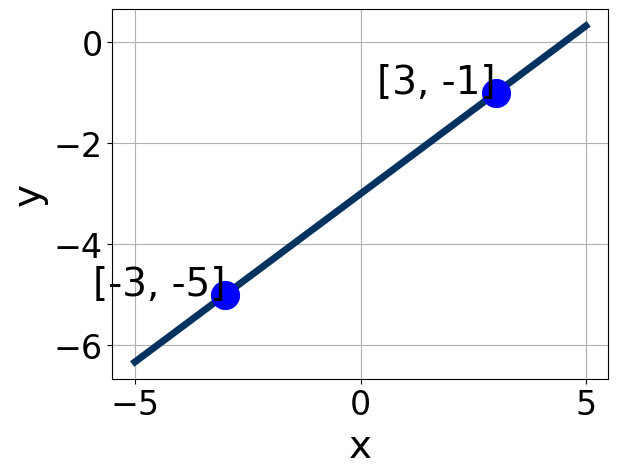
\includegraphics[width=0.5\textwidth]{../Figures/linearGraphToStandardB.png}
\end{center}
\begin{enumerate}[label=\Alph*.]
\item \( A \in [-1.1, 0.8], \hspace{3mm} B \in [-1.19, -0.36], \text{ and } \hspace{3mm} C \in [3, 5] \)
\item \( A \in [0.2, 4.6], \hspace{3mm} B \in [-3.08, -2.05], \text{ and } \hspace{3mm} C \in [6, 10] \)
\item \( A \in [-1.1, 0.8], \hspace{3mm} B \in [0.89, 1.62], \text{ and } \hspace{3mm} C \in [-8, -2] \)
\item \( A \in [-5.8, -0.7], \hspace{3mm} B \in [2.8, 3.32], \text{ and } \hspace{3mm} C \in [-11, -7] \)
\item \( A \in [0.2, 4.6], \hspace{3mm} B \in [2.8, 3.32], \text{ and } \hspace{3mm} C \in [-11, -7] \)

\end{enumerate} }
\litem{
First, find the equation of the line containing the two points below. Then, write the equation as $ y=mx+b $ and choose the intervals that contain $m$ and $b$.\[ (5, 3) \text{ and } (11, 10) \]\begin{enumerate}[label=\Alph*.]
\item \( m \in [-0.83, 6.17] \hspace*{3mm} b \in [-2.54, -1.8] \)
\item \( m \in [-1.17, -0.17] \hspace*{3mm} b \in [22.14, 23.51] \)
\item \( m \in [-0.83, 6.17] \hspace*{3mm} b \in [-3.07, -2.42] \)
\item \( m \in [-0.83, 6.17] \hspace*{3mm} b \in [2.6, 2.94] \)
\item \( m \in [-0.83, 6.17] \hspace*{3mm} b \in [-1.18, -0.59] \)

\end{enumerate} }
\litem{
Find the equation of the line described below. Write the linear equation as $ y=mx+b $ and choose the intervals that contain $m$ and $b$.\[ \text{Perpendicular to } 9 x + 8 y = 11 \text{ and passing through the point } (-7, -3). \]\begin{enumerate}[label=\Alph*.]
\item \( m \in [0.71, 1.08] \hspace*{3mm} b \in [-4, -2.7] \)
\item \( m \in [0.71, 1.08] \hspace*{3mm} b \in [2.4, 3.5] \)
\item \( m \in [0.71, 1.08] \hspace*{3mm} b \in [3.9, 5.3] \)
\item \( m \in [-1.52, -0.72] \hspace*{3mm} b \in [-10.2, -8.8] \)
\item \( m \in [1.01, 1.65] \hspace*{3mm} b \in [2.4, 3.5] \)

\end{enumerate} }
\litem{
Solve the linear equation below. Then, choose the interval that contains the solution.\[ \frac{7x -3}{8} - \frac{7x -8}{6} = \frac{-6x -4}{7} \]\begin{enumerate}[label=\Alph*.]
\item \( x \in [-0.9, -0.1] \)
\item \( x \in [-3.1, -1] \)
\item \( x \in [-16.3, -15.8] \)
\item \( x \in [1.2, 2.1] \)
\item \( \text{There are no real solutions.} \)

\end{enumerate} }
\end{enumerate}

\end{document}